%------------------------------------------------------------
% thesis completion seminar - Andy Taylor 
%------------------------------------------------------------
\documentclass{beamer}
\usepackage[utf8]{inputenc}
\usepackage{style/uom_beamer}

%\newcommand{\figureInit}{\begin{figure}[h]\centering}
%------------------------------------------------------------------------ 
% shortcut text
%------------------------------------------------------------------------ 
\newcommand{\TITLE}{`TITLE'}
\newcommand{\ALTTITLE}{`ALT TITLE'}
\newcommand{\BOM}{Australian Bureau of Meteorology}
\newcommand{\LTE}{\textbf{\texttt{LTE}}}
\newcommand{\ATGF}{\textbf{\texttt{ATGF}}}
\newcommand{\ATGP}{\textbf{\texttt{ATGP}}}
\newcommand{\SSH}{\textbf{\texttt{ssh}}}
\newcommand{\BL}{\textbf{\texttt{Bluelink-OceanMAPS}}}
\newcommand{\MOM}{\textbf{\texttt{MOM}}}
\newcommand{\ROMS}{\textbf{\texttt{ROMS}}}
\newcommand{\GODAE}{\textbf{\texttt{GODAE}}}
\newcommand{\OGCM}{\textbf{\texttt{{OGCM}}}}       %{\textbf{\texttt{OGCM}}}
\newcommand{\OFAM}{\textbf{\texttt{{OFAM}}}}
\newcommand{\OFAMHR}{\textbf{\texttt{{OFAMHR}}}}
\newcommand{\NWP}{\textbf{\texttt{NWP}}}
\newcommand{\OTIS}{\textbf{\texttt{OTIS}}}
\newcommand{\GOOS}{\textbf{\texttt{GOOS}}}
\newcommand{\obc}{\textbf{\texttt{obc}}}
\newcommand{\ANTT}{\textbf{\texttt{ANTT}}}
\newcommand{\CTE}{\textbf{\texttt{CTE}}}
\newcommand{\SAL}{\textbf{\texttt{SAL}}}
\newcommand{\AG}{\textbf{\texttt{ACCESS-G}}}
\newcommand{\AR}{\textbf{\texttt{ACCESS-R}}}
\newcommand{\ER}{\textbf{\texttt{eReefs}}}

% add DRAFT water mark
\usepackage{draftwatermark}
\SetWatermarkText{DRAFT} 
\SetWatermarkLightness{0.98}
\SetWatermarkAngle{45}
\SetWatermarkScale{1.2}
                % draft watermark
\begin{document}
%------------------------------------------------------------
% metadata  ..note syntax: [short]{long}
\title[Tides and sea level forecasting]{On the application of conventional tidal concepts within operational sea level forecasting}
\author[Andy Taylor]{Andy Taylor} 
\newcommand{\department}{School of Earth Sciences}
\newcommand{\university}{\textsc{The University of Melbourne}}
\newcommand{\BoM}{\sc Australian Bureau of Meteorology}
\institute[]{\university \par \department  \par and \par \BoM}
\date[Completion 2021]{Completion Seminar 21-03-2021}
%------------------------------------------------------------
% title slide 
\frame{\titlepage}
%------------------------------------------------------------
% auto overview for every section in style file
%------------------------------------------------------------
% sections 
\section{Summary}
\begin{frame}
\frametitle{Abstract}

Part-time thesis with publication:
\begin{itemize}
    \item conceptual intersection of tides and mesoscale oceanography
    \item motivation towards \bold{seamless} forecasting
    \item background of simulation system upgrades
    \item new methods for combining, evaluating and delivering nominally ``tidal'' sea level information
    \item focus on representation and incompatibility
     updates 
\end{itemize}

\end{frame}

\section{Intro}
\begin{frame}
\frametitle{Brief intro yarn}
Super brief personal story.

Why this topic?

% ;prelude 1:  the perspnal yarn
% renewables,  fluids - HPS
% travel 
% sailing pelican -> antt!
% naval engineering -> renewables
% BoM encounters
% ...wind obs for bankable truth
% ...ocean forecasts -> but 'nontidal'!?
% Academic
% ...wave interest via offshore -> AlexB
% ...reality $$ job or scholarship
% Bluelink
% ...inherit sea level report
% ...expand 

\end{frame}
\begin{frame}
\frametitle{Historical context}

Tides and forecasting
analysis 
tide tables
laws and convention


NWP
satellites
godae
altimeters
data assimilation


satellites
tides 
orbits
corrections


government
'official'
references
services

\end{frame}
%-----------------------------------------
\begin{frame}
\frametitle{Motivating applications}
\begin{minipage}{0.45\textwidth}
    \begin{figure}      
    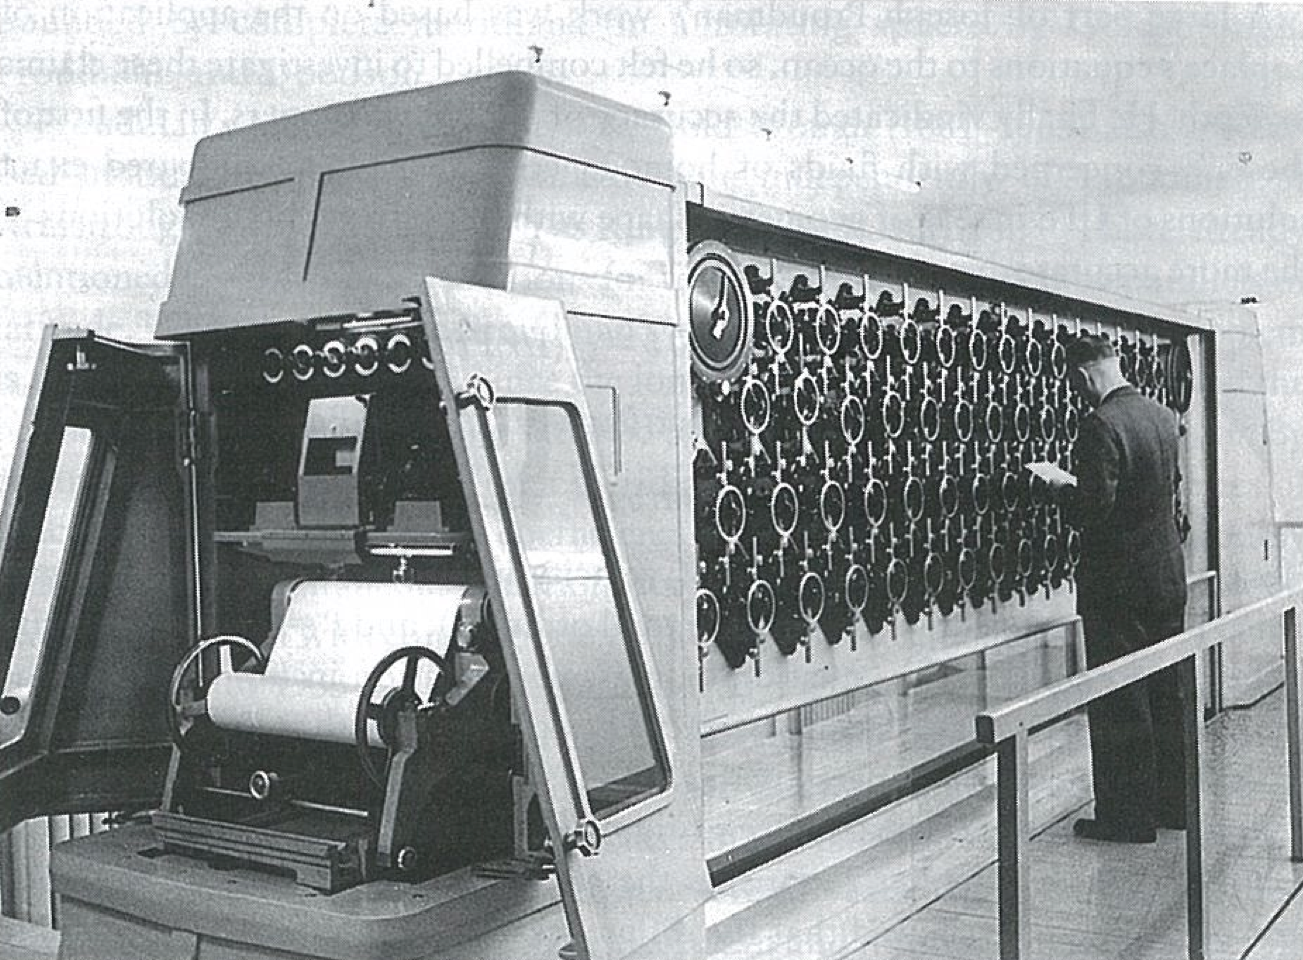
\includegraphics[width=\textwidth]{figures/images/DHI_machine_cartwright_fig11p2.png}
    \end{figure}
\end{minipage}
\hfill
\begin{minipage}{0.45\textwidth}
    Some text here.
\end{minipage}
\end{frame}
%-----------------------------------------
%--------
\section{Tides}
\begin{frame}
\frametitle{Sample frame title}

\end{frame}
\begin{frame}
\frametitle{Sample frame title}

\end{frame}
\begin{frame}
\frametitle{Sample frame title}

\end{frame}
%--------
\section{}
\begin{frame}
\frametitle{Questions}
Thanks

\end{frame}

%------------------------------------------------------------
\end{document}



